\documentclass[1p]{elsarticle_modified}
%\bibliographystyle{elsarticle-num}

%\usepackage[colorlinks]{hyperref}
%\usepackage{abbrmath_seonhwa} %\Abb, \Ascr, \Acal ,\Abf, \Afrak
\usepackage{amsfonts}
\usepackage{amssymb}
\usepackage{amsmath}
\usepackage{amsthm}
\usepackage{scalefnt}
\usepackage{amsbsy}
\usepackage{kotex}
\usepackage{caption}
\usepackage{subfig}
\usepackage{color}
\usepackage{graphicx}
\usepackage{xcolor} %% white, black, red, green, blue, cyan, magenta, yellow
\usepackage{float}
\usepackage{setspace}
\usepackage{hyperref}

\usepackage{tikz}
\usetikzlibrary{arrows}

\usepackage{multirow}
\usepackage{array} % fixed length table
\usepackage{hhline}

%%%%%%%%%%%%%%%%%%%%%
\makeatletter
\renewcommand*\env@matrix[1][\arraystretch]{%
	\edef\arraystretch{#1}%
	\hskip -\arraycolsep
	\let\@ifnextchar\new@ifnextchar
	\array{*\c@MaxMatrixCols c}}
\makeatother %https://tex.stackexchange.com/questions/14071/how-can-i-increase-the-line-spacing-in-a-matrix
%%%%%%%%%%%%%%%

\usepackage[normalem]{ulem}

\newcommand{\msout}[1]{\ifmmode\text{\sout{\ensuremath{#1}}}\else\sout{#1}\fi}
%SOURCE: \msout is \stkout macro in https://tex.stackexchange.com/questions/20609/strikeout-in-math-mode

\newcommand{\cancel}[1]{
	\ifmmode
	{\color{red}\msout{#1}}
	\else
	{\color{red}\sout{#1}}
	\fi
}

\newcommand{\add}[1]{
	{\color{blue}\uwave{#1}}
}

\newcommand{\replace}[2]{
	\ifmmode
	{\color{red}\msout{#1}}{\color{blue}\uwave{#2}}
	\else
	{\color{red}\sout{#1}}{\color{blue}\uwave{#2}}
	\fi
}

\newcommand{\Sol}{\mathcal{S}} %segment
\newcommand{\D}{D} %diagram
\newcommand{\A}{\mathcal{A}} %arc


%%%%%%%%%%%%%%%%%%%%%%%%%%%%%5 test

\def\sl{\operatorname{\textup{SL}}(2,\Cbb)}
\def\psl{\operatorname{\textup{PSL}}(2,\Cbb)}
\def\quan{\mkern 1mu \triangleright \mkern 1mu}

\theoremstyle{definition}
\newtheorem{thm}{Theorem}[section]
\newtheorem{prop}[thm]{Proposition}
\newtheorem{lem}[thm]{Lemma}
\newtheorem{ques}[thm]{Question}
\newtheorem{cor}[thm]{Corollary}
\newtheorem{defn}[thm]{Definition}
\newtheorem{exam}[thm]{Example}
\newtheorem{rmk}[thm]{Remark}
\newtheorem{alg}[thm]{Algorithm}

\newcommand{\I}{\sqrt{-1}}
\begin{document}

%\begin{frontmatter}
%
%\title{Boundary parabolic representations of knots up to 8 crossings}
%
%%% Group authors per affiliation:
%\author{Yunhi Cho} 
%\address{Department of Mathematics, University of Seoul, Seoul, Korea}
%\ead{yhcho@uos.ac.kr}
%
%
%\author{Seonhwa Kim} %\fnref{s_kim}}
%\address{Center for Geometry and Physics, Institute for Basic Science, Pohang, 37673, Korea}
%\ead{ryeona17@ibs.re.kr}
%
%\author{Hyuk Kim}
%\address{Department of Mathematical Sciences, Seoul National University, Seoul 08826, Korea}
%\ead{hyukkim@snu.ac.kr}
%
%\author{Seokbeom Yoon}
%\address{Department of Mathematical Sciences, Seoul National University, Seoul, 08826,  Korea}
%\ead{sbyoon15@snu.ac.kr}
%
%\begin{abstract}
%We find all boundary parabolic representation of knots up to 8 crossings.
%
%\end{abstract}
%\begin{keyword}
%    \MSC[2010] 57M25 
%\end{keyword}
%
%\end{frontmatter}

%\linenumbers
%\tableofcontents
%
\newcommand\colored[1]{\textcolor{white}{\rule[-0.35ex]{0.8em}{1.4ex}}\kern-0.8em\color{red} #1}%
%\newcommand\colored[1]{\textcolor{white}{ #1}\kern-2.17ex	\textcolor{white}{ #1}\kern-1.81ex	\textcolor{white}{ #1}\kern-2.15ex\color{red}#1	}

{\Large $\underline{12a_{0620}~(K12a_{0620})}$}

\setlength{\tabcolsep}{10pt}
\renewcommand{\arraystretch}{1.6}
\vspace{1cm}\begin{tabular}{m{100pt}>{\centering\arraybackslash}m{274pt}}
\multirow{5}{120pt}{
	\centering
	\includegraphics[width=112pt]{../../../GIT/diagram.site/Diagrams/png/1421_12a_0620.png}\\
\ \ \ A knot diagram\footnotemark}&
\allowdisplaybreaks
\textbf{Linearized knot diagam} \\
\cline{2-2}
 &
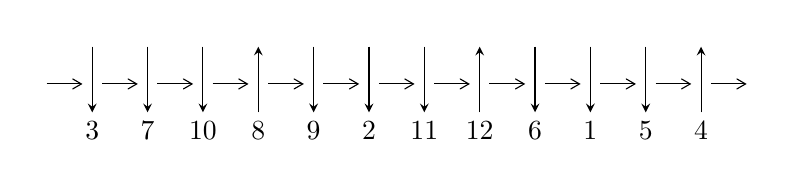
\begin{tikzpicture}[x=20pt, y=17pt]
	% nodes
	\node (C0) at (0, 0) {};
	\node (C1) at (1, 0) {};
	\node (C1U) at (1, +1) {};
	\node (C1D) at (1, -1) {3};

	\node (C2) at (2, 0) {};
	\node (C2U) at (2, +1) {};
	\node (C2D) at (2, -1) {7};

	\node (C3) at (3, 0) {};
	\node (C3U) at (3, +1) {};
	\node (C3D) at (3, -1) {10};

	\node (C4) at (4, 0) {};
	\node (C4U) at (4, +1) {};
	\node (C4D) at (4, -1) {8};

	\node (C5) at (5, 0) {};
	\node (C5U) at (5, +1) {};
	\node (C5D) at (5, -1) {9};

	\node (C6) at (6, 0) {};
	\node (C6U) at (6, +1) {};
	\node (C6D) at (6, -1) {2};

	\node (C7) at (7, 0) {};
	\node (C7U) at (7, +1) {};
	\node (C7D) at (7, -1) {11};

	\node (C8) at (8, 0) {};
	\node (C8U) at (8, +1) {};
	\node (C8D) at (8, -1) {12};

	\node (C9) at (9, 0) {};
	\node (C9U) at (9, +1) {};
	\node (C9D) at (9, -1) {6};

	\node (C10) at (10, 0) {};
	\node (C10U) at (10, +1) {};
	\node (C10D) at (10, -1) {1};

	\node (C11) at (11, 0) {};
	\node (C11U) at (11, +1) {};
	\node (C11D) at (11, -1) {5};

	\node (C12) at (12, 0) {};
	\node (C12U) at (12, +1) {};
	\node (C12D) at (12, -1) {4};
	\node (C13) at (13, 0) {};

	% arrows
	\draw[->,>={angle 60}]
	(C0) edge (C1) (C1) edge (C2) (C2) edge (C3) (C3) edge (C4) (C4) edge (C5) (C5) edge (C6) (C6) edge (C7) (C7) edge (C8) (C8) edge (C9) (C9) edge (C10) (C10) edge (C11) (C11) edge (C12) (C12) edge (C13) ;	\draw[->,>=stealth]
	(C1U) edge (C1D) (C2U) edge (C2D) (C3U) edge (C3D) (C4D) edge (C4U) (C5U) edge (C5D) (C6U) edge (C6D) (C7U) edge (C7D) (C8D) edge (C8U) (C9U) edge (C9D) (C10U) edge (C10D) (C11U) edge (C11D) (C12D) edge (C12U) ;
	\end{tikzpicture} \\
\hhline{~~} \\& 
\textbf{Solving Sequence} \\ \cline{2-2} 
 &
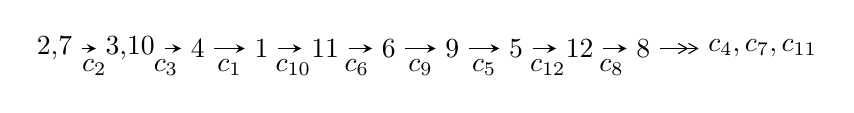
\begin{tikzpicture}[x=23pt, y=7pt]
	% node
	\node (A0) at (-1/8, 0) {2,7};
	\node (A1) at (17/16, 0) {3,10};
	\node (A2) at (17/8, 0) {4};
	\node (A3) at (25/8, 0) {1};
	\node (A4) at (33/8, 0) {11};
	\node (A5) at (41/8, 0) {6};
	\node (A6) at (49/8, 0) {9};
	\node (A7) at (57/8, 0) {5};
	\node (A8) at (65/8, 0) {12};
	\node (A9) at (73/8, 0) {8};
	\node (C1) at (1/2, -1) {$c_{2}$};
	\node (C2) at (13/8, -1) {$c_{3}$};
	\node (C3) at (21/8, -1) {$c_{1}$};
	\node (C4) at (29/8, -1) {$c_{10}$};
	\node (C5) at (37/8, -1) {$c_{6}$};
	\node (C6) at (45/8, -1) {$c_{9}$};
	\node (C7) at (53/8, -1) {$c_{5}$};
	\node (C8) at (61/8, -1) {$c_{12}$};
	\node (C9) at (69/8, -1) {$c_{8}$};
	\node (A10) at (11, 0) {$c_{4},c_{7},c_{11}$};

	% edge
	\draw[->,>=stealth]	
	(A0) edge (A1) (A1) edge (A2) (A2) edge (A3) (A3) edge (A4) (A4) edge (A5) (A5) edge (A6) (A6) edge (A7) (A7) edge (A8) (A8) edge (A9) ;
	\draw[->>,>={angle 60}]	
	(A9) edge (A10);
\end{tikzpicture} \\ 

\end{tabular} \\

\footnotetext{
The image of knot diagram is generated by the software ``\textbf{Draw programme}" developed by Andrew Bartholomew(\url{http://www.layer8.co.uk/maths/draw/index.htm\#Running-draw}), where we modified some parts for our purpose(\url{https://github.com/CATsTAILs/LinksPainter}).
}\phantom \\ \newline 
\centering \textbf{Ideals for irreducible components\footnotemark of $X_{\text{par}}$} 
 
\begin{align*}
I^u_{1}&=\langle 
-2.08101\times10^{510} u^{166}-1.11697\times10^{510} u^{165}+\cdots+2.56234\times10^{507} b-1.20192\times10^{512},\\
\phantom{I^u_{1}}&\phantom{= \langle  }-6.65713\times10^{511} u^{166}-3.56687\times10^{511} u^{165}+\cdots+7.94327\times10^{508} a-3.84871\times10^{513},\\
\phantom{I^u_{1}}&\phantom{= \langle  }u^{167}-37 u^{165}+\cdots+29 u-31\rangle \\
I^u_{2}&=\langle 
1594092397 u^{32}+83351656 u^{31}+\cdots+135513403 b+2264420315,\\
\phantom{I^u_{2}}&\phantom{= \langle  }1580036566 u^{32}+229087797 u^{31}+\cdots+135513403 a+1642262255,\;u^{33}- u^{32}+\cdots+4 u-1\rangle \\
\\
\end{align*}
\raggedright * 2 irreducible components of $\dim_{\mathbb{C}}=0$, with total 200 representations.\\
\footnotetext{All coefficients of polynomials are rational numbers. But the coefficients are sometimes approximated in decimal forms when there is not enough margin.}
\newpage
\renewcommand{\arraystretch}{1}
\centering \section*{I. $I^u_{1}= \langle -2.08\times10^{510} u^{166}-1.12\times10^{510} u^{165}+\cdots+2.56\times10^{507} b-1.20\times10^{512},\;-6.66\times10^{511} u^{166}-3.57\times10^{511} u^{165}+\cdots+7.94\times10^{508} a-3.85\times10^{513},\;u^{167}-37 u^{165}+\cdots+29 u-31 \rangle$}
\flushleft \textbf{(i) Arc colorings}\\
\begin{tabular}{m{7pt} m{180pt} m{7pt} m{180pt} }
\flushright $a_{2}=$&$\begin{pmatrix}1\\0\end{pmatrix}$ \\
\flushright $a_{7}=$&$\begin{pmatrix}0\\u\end{pmatrix}$ \\
\flushright $a_{3}=$&$\begin{pmatrix}1\\u^2\end{pmatrix}$ \\
\flushright $a_{10}=$&$\begin{pmatrix}838.084 u^{166}+449.043 u^{165}+\cdots+44952.3 u+48452.5\\812.152 u^{166}+435.919 u^{165}+\cdots+43482.7 u+46907.0\end{pmatrix}$ \\
\flushright $a_{4}=$&$\begin{pmatrix}-238.456 u^{166}-127.353 u^{165}+\cdots-13117.7 u-13893.0\\-623.598 u^{166}-334.543 u^{165}+\cdots-33581.9 u-36074.6\end{pmatrix}$ \\
\flushright $a_{1}=$&$\begin{pmatrix}- u^2+1\\- u^4\end{pmatrix}$ \\
\flushright $a_{11}=$&$\begin{pmatrix}377.436 u^{166}+201.932 u^{165}+\cdots+20262.8 u+21837.5\\865.582 u^{166}+464.572 u^{165}+\cdots+46356.2 u+49996.8\end{pmatrix}$ \\
\flushright $a_{6}=$&$\begin{pmatrix}u\\u\end{pmatrix}$ \\
\flushright $a_{9}=$&$\begin{pmatrix}831.803 u^{166}+446.225 u^{165}+\cdots+44529.0 u+48045.6\\805.870 u^{166}+433.100 u^{165}+\cdots+43059.4 u+46500.2\end{pmatrix}$ \\
\flushright $a_{5}=$&$\begin{pmatrix}308.322 u^{166}+164.498 u^{165}+\cdots+16672.3 u+17886.8\\291.773 u^{166}+156.972 u^{165}+\cdots+15574.2 u+16842.4\end{pmatrix}$ \\
\flushright $a_{12}=$&$\begin{pmatrix}616.362 u^{166}+331.540 u^{165}+\cdots+32808.7 u+35502.4\\1106.39 u^{166}+593.646 u^{165}+\cdots+59276.4 u+63912.1\end{pmatrix}$ \\
\flushright $a_{8}=$&$\begin{pmatrix}-189.071 u^{166}-99.8465 u^{165}+\cdots-10407.2 u-11055.9\\-133.267 u^{166}-70.7867 u^{165}+\cdots-7253.57 u-7765.33\end{pmatrix}$\\&\end{tabular}
\flushleft \textbf{(ii) Obstruction class $= -1$}\\~\\
\flushleft \textbf{(iii) Cusp Shapes $= -1360.90 u^{166}-729.931 u^{165}+\cdots-72748.9 u-78562.5$}\\~\\
\newpage\renewcommand{\arraystretch}{1}
\flushleft \textbf{(iv) u-Polynomials at the component}\newline \\
\begin{tabular}{m{50pt}|m{274pt}}
Crossings & \hspace{64pt}u-Polynomials at each crossing \\
\hline $$\begin{aligned}c_{1}\end{aligned}$$&$\begin{aligned}
&u^{167}+74 u^{166}+\cdots+31221 u+961
\end{aligned}$\\
\hline $$\begin{aligned}c_{2},c_{6}\end{aligned}$$&$\begin{aligned}
&u^{167}-37 u^{165}+\cdots+29 u-31
\end{aligned}$\\
\hline $$\begin{aligned}c_{3}\end{aligned}$$&$\begin{aligned}
&u^{167}-14 u^{165}+\cdots+135699 u+7999
\end{aligned}$\\
\hline $$\begin{aligned}c_{4}\end{aligned}$$&$\begin{aligned}
&u^{167}+2 u^{166}+\cdots-13 u-1
\end{aligned}$\\
\hline $$\begin{aligned}c_{5},c_{9}\end{aligned}$$&$\begin{aligned}
&u^{167}+4 u^{166}+\cdots-100431668 u-12620969
\end{aligned}$\\
\hline $$\begin{aligned}c_{7}\end{aligned}$$&$\begin{aligned}
&u^{167}-4 u^{166}+\cdots-42690283337 u-34553045579
\end{aligned}$\\
\hline $$\begin{aligned}c_{8}\end{aligned}$$&$\begin{aligned}
&u^{167}+3 u^{166}+\cdots+2613531 u+97585
\end{aligned}$\\
\hline $$\begin{aligned}c_{10}\end{aligned}$$&$\begin{aligned}
&u^{167}+12 u^{166}+\cdots+35 u-1
\end{aligned}$\\
\hline $$\begin{aligned}c_{11}\end{aligned}$$&$\begin{aligned}
&u^{167}+5 u^{166}+\cdots-119637 u+24543
\end{aligned}$\\
\hline $$\begin{aligned}c_{12}\end{aligned}$$&$\begin{aligned}
&u^{167}+12 u^{166}+\cdots+526426257314 u+56057085917
\end{aligned}$\\
\hline
\end{tabular}\\~\\
\newpage\renewcommand{\arraystretch}{1}
\flushleft \textbf{(v) Riley Polynomials at the component}\newline \\
\begin{tabular}{m{50pt}|m{274pt}}
Crossings & \hspace{64pt}Riley Polynomials at each crossing \\
\hline $$\begin{aligned}c_{1}\end{aligned}$$&$\begin{aligned}
&y^{167}+30 y^{166}+\cdots-77198199 y-923521
\end{aligned}$\\
\hline $$\begin{aligned}c_{2},c_{6}\end{aligned}$$&$\begin{aligned}
&y^{167}-74 y^{166}+\cdots+31221 y-961
\end{aligned}$\\
\hline $$\begin{aligned}c_{3}\end{aligned}$$&$\begin{aligned}
&y^{167}-28 y^{166}+\cdots+27826081971 y-63984001
\end{aligned}$\\
\hline $$\begin{aligned}c_{4}\end{aligned}$$&$\begin{aligned}
&y^{167}+64 y^{166}+\cdots-11 y-1
\end{aligned}$\\
\hline $$\begin{aligned}c_{5},c_{9}\end{aligned}$$&$\begin{aligned}
&y^{167}-102 y^{166}+\cdots+847414145497076 y-159288858498961
\end{aligned}$\\
\hline $$\begin{aligned}c_{7}\end{aligned}$$&$\begin{aligned}
&y^{167}-80 y^{166}+\cdots+8.05\times10^{22} y-1.19\times10^{21}
\end{aligned}$\\
\hline $$\begin{aligned}c_{8}\end{aligned}$$&$\begin{aligned}
&y^{167}+49 y^{166}+\cdots-1685246559 y-9522832225
\end{aligned}$\\
\hline $$\begin{aligned}c_{10}\end{aligned}$$&$\begin{aligned}
&y^{167}-58 y^{166}+\cdots+67 y-1
\end{aligned}$\\
\hline $$\begin{aligned}c_{11}\end{aligned}$$&$\begin{aligned}
&y^{167}-41 y^{166}+\cdots+36907101225 y-602358849
\end{aligned}$\\
\hline $$\begin{aligned}c_{12}\end{aligned}$$&$\begin{aligned}
&y^{167}+76 y^{166}+\cdots-1.98\times10^{23} y-3.14\times10^{21}
\end{aligned}$\\
\hline
\end{tabular}\\~\\
\newpage\flushleft \textbf{(vi) Complex Volumes and Cusp Shapes}
$$\begin{array}{c|c|c}  
\text{Solutions to }I^u_{1}& \I (\text{vol} + \sqrt{-1}CS) & \text{Cusp shape}\\
 \hline 
\begin{aligned}
u &= -0.408975 + 0.915806 I \\
a &= \phantom{-}1.14813 + 1.07154 I \\
b &= \phantom{-}1.056770 - 0.592885 I\end{aligned}
 & -4.85860 - 6.29115 I & \phantom{-0.000000 } 0 \\ \hline\begin{aligned}
u &= -0.408975 - 0.915806 I \\
a &= \phantom{-}1.14813 - 1.07154 I \\
b &= \phantom{-}1.056770 + 0.592885 I\end{aligned}
 & -4.85860 + 6.29115 I & \phantom{-0.000000 } 0 \\ \hline\begin{aligned}
u &= \phantom{-}0.992444 + 0.165700 I \\
a &= -1.04664 + 1.19512 I \\
b &= -0.702766 + 0.724377 I\end{aligned}
 & -4.74546 + 1.25465 I & \phantom{-0.000000 } 0 \\ \hline\begin{aligned}
u &= \phantom{-}0.992444 - 0.165700 I \\
a &= -1.04664 - 1.19512 I \\
b &= -0.702766 - 0.724377 I\end{aligned}
 & -4.74546 - 1.25465 I & \phantom{-0.000000 } 0 \\ \hline\begin{aligned}
u &= \phantom{-}0.749312 + 0.643529 I \\
a &= \phantom{-}0.598920 - 1.030590 I \\
b &= \phantom{-}1.142340 - 0.634546 I\end{aligned}
 & \phantom{-}2.27307 - 2.26166 I & \phantom{-0.000000 } 0 \\ \hline\begin{aligned}
u &= \phantom{-}0.749312 - 0.643529 I \\
a &= \phantom{-}0.598920 + 1.030590 I \\
b &= \phantom{-}1.142340 + 0.634546 I\end{aligned}
 & \phantom{-}2.27307 + 2.26166 I & \phantom{-0.000000 } 0 \\ \hline\begin{aligned}
u &= \phantom{-}0.619664 + 0.809985 I \\
a &= -1.79866 + 0.24946 I \\
b &= -1.21545 - 0.83450 I\end{aligned}
 & -0.97974 + 4.90783 I & \phantom{-0.000000 } 0 \\ \hline\begin{aligned}
u &= \phantom{-}0.619664 - 0.809985 I \\
a &= -1.79866 - 0.24946 I \\
b &= -1.21545 + 0.83450 I\end{aligned}
 & -0.97974 - 4.90783 I & \phantom{-0.000000 } 0 \\ \hline\begin{aligned}
u &= -0.215636 + 0.955936 I \\
a &= -0.462979 - 1.195860 I \\
b &= -0.459418 + 0.084270 I\end{aligned}
 & \phantom{-}0.10022 - 6.05933 I & \phantom{-0.000000 } 0 \\ \hline\begin{aligned}
u &= -0.215636 - 0.955936 I \\
a &= -0.462979 + 1.195860 I \\
b &= -0.459418 - 0.084270 I\end{aligned}
 & \phantom{-}0.10022 + 6.05933 I & \phantom{-0.000000 } 0\\
 \hline 
 \end{array}$$\newpage$$\begin{array}{c|c|c}  
\text{Solutions to }I^u_{1}& \I (\text{vol} + \sqrt{-1}CS) & \text{Cusp shape}\\
 \hline 
\begin{aligned}
u &= -0.556073 + 0.796049 I \\
a &= \phantom{-}1.19285 + 0.81528 I \\
b &= \phantom{-}0.701546 - 0.348352 I\end{aligned}
 & -0.92725 - 1.10901 I & \phantom{-0.000000 } 0 \\ \hline\begin{aligned}
u &= -0.556073 - 0.796049 I \\
a &= \phantom{-}1.19285 - 0.81528 I \\
b &= \phantom{-}0.701546 + 0.348352 I\end{aligned}
 & -0.92725 + 1.10901 I & \phantom{-0.000000 } 0 \\ \hline\begin{aligned}
u &= \phantom{-}0.404589 + 0.947213 I \\
a &= \phantom{-}1.15466 - 0.99311 I \\
b &= \phantom{-}1.024780 + 0.535124 I\end{aligned}
 & -5.1206 + 15.0097 I & \phantom{-0.000000 } 0 \\ \hline\begin{aligned}
u &= \phantom{-}0.404589 - 0.947213 I \\
a &= \phantom{-}1.15466 + 0.99311 I \\
b &= \phantom{-}1.024780 - 0.535124 I\end{aligned}
 & -5.1206 - 15.0097 I & \phantom{-0.000000 } 0 \\ \hline\begin{aligned}
u &= \phantom{-}0.860711 + 0.440907 I \\
a &= -3.18176 + 2.75428 I \\
b &= -3.56155 - 0.47510 I\end{aligned}
 & -3.47103 - 1.84047 I & \phantom{-0.000000 } 0 \\ \hline\begin{aligned}
u &= \phantom{-}0.860711 - 0.440907 I \\
a &= -3.18176 - 2.75428 I \\
b &= -3.56155 + 0.47510 I\end{aligned}
 & -3.47103 + 1.84047 I & \phantom{-0.000000 } 0 \\ \hline\begin{aligned}
u &= -0.442760 + 0.857409 I \\
a &= \phantom{-}0.296060 - 0.978793 I \\
b &= -0.425478 - 0.455941 I\end{aligned}
 & \phantom{-}0.30104 + 5.37087 I & \phantom{-0.000000 } 0 \\ \hline\begin{aligned}
u &= -0.442760 - 0.857409 I \\
a &= \phantom{-}0.296060 + 0.978793 I \\
b &= -0.425478 + 0.455941 I\end{aligned}
 & \phantom{-}0.30104 - 5.37087 I & \phantom{-0.000000 } 0 \\ \hline\begin{aligned}
u &= \phantom{-}0.946569 + 0.426333 I \\
a &= -0.69093 + 1.64490 I \\
b &= -2.11899 + 1.73351 I\end{aligned}
 & -3.90035 - 1.31681 I & \phantom{-0.000000 } 0 \\ \hline\begin{aligned}
u &= \phantom{-}0.946569 - 0.426333 I \\
a &= -0.69093 - 1.64490 I \\
b &= -2.11899 - 1.73351 I\end{aligned}
 & -3.90035 + 1.31681 I & \phantom{-0.000000 } 0\\
 \hline 
 \end{array}$$\newpage$$\begin{array}{c|c|c}  
\text{Solutions to }I^u_{1}& \I (\text{vol} + \sqrt{-1}CS) & \text{Cusp shape}\\
 \hline 
\begin{aligned}
u &= -0.864166 + 0.406390 I \\
a &= \phantom{-}2.81837 + 2.98326 I \\
b &= \phantom{-}3.58600 - 0.33116 I\end{aligned}
 & -3.54493 + 1.73658 I & \phantom{-0.000000 } 0 \\ \hline\begin{aligned}
u &= -0.864166 - 0.406390 I \\
a &= \phantom{-}2.81837 - 2.98326 I \\
b &= \phantom{-}3.58600 + 0.33116 I\end{aligned}
 & -3.54493 - 1.73658 I & \phantom{-0.000000 } 0 \\ \hline\begin{aligned}
u &= -0.697874 + 0.648649 I \\
a &= -0.650486 + 0.406485 I \\
b &= \phantom{-}0.068524 + 1.225080 I\end{aligned}
 & -1.67902 + 3.41376 I & \phantom{-0.000000 } 0 \\ \hline\begin{aligned}
u &= -0.697874 - 0.648649 I \\
a &= -0.650486 - 0.406485 I \\
b &= \phantom{-}0.068524 - 1.225080 I\end{aligned}
 & -1.67902 - 3.41376 I & \phantom{-0.000000 } 0 \\ \hline\begin{aligned}
u &= -0.498692 + 0.804668 I \\
a &= \phantom{-}0.542602 + 1.108590 I \\
b &= \phantom{-}1.51627 + 0.09936 I\end{aligned}
 & \phantom{-}0.59250 - 8.86800 I & \phantom{-0.000000 } 0 \\ \hline\begin{aligned}
u &= -0.498692 - 0.804668 I \\
a &= \phantom{-}0.542602 - 1.108590 I \\
b &= \phantom{-}1.51627 - 0.09936 I\end{aligned}
 & \phantom{-}0.59250 + 8.86800 I & \phantom{-0.000000 } 0 \\ \hline\begin{aligned}
u &= \phantom{-}0.454082 + 0.829965 I \\
a &= -0.055302 + 0.654540 I \\
b &= -0.739473 + 0.422648 I\end{aligned}
 & \phantom{-}3.52312 + 2.60647 I & \phantom{-0.000000 } 0 \\ \hline\begin{aligned}
u &= \phantom{-}0.454082 - 0.829965 I \\
a &= -0.055302 - 0.654540 I \\
b &= -0.739473 - 0.422648 I\end{aligned}
 & \phantom{-}3.52312 - 2.60647 I & \phantom{-0.000000 } 0 \\ \hline\begin{aligned}
u &= \phantom{-}0.993976 + 0.351859 I \\
a &= \phantom{-}0.539564 + 1.197380 I \\
b &= \phantom{-}1.72459 + 0.59899 I\end{aligned}
 & -7.67265 - 0.06243 I & \phantom{-0.000000 } 0 \\ \hline\begin{aligned}
u &= \phantom{-}0.993976 - 0.351859 I \\
a &= \phantom{-}0.539564 - 1.197380 I \\
b &= \phantom{-}1.72459 - 0.59899 I\end{aligned}
 & -7.67265 + 0.06243 I & \phantom{-0.000000 } 0\\
 \hline 
 \end{array}$$\newpage$$\begin{array}{c|c|c}  
\text{Solutions to }I^u_{1}& \I (\text{vol} + \sqrt{-1}CS) & \text{Cusp shape}\\
 \hline 
\begin{aligned}
u &= \phantom{-}0.526130 + 0.776524 I \\
a &= \phantom{-}0.812429 - 0.979816 I \\
b &= \phantom{-}1.122510 - 0.055505 I\end{aligned}
 & \phantom{-}4.04239 + 0.69020 I & \phantom{-0.000000 } 0 \\ \hline\begin{aligned}
u &= \phantom{-}0.526130 - 0.776524 I \\
a &= \phantom{-}0.812429 + 0.979816 I \\
b &= \phantom{-}1.122510 + 0.055505 I\end{aligned}
 & \phantom{-}4.04239 - 0.69020 I & \phantom{-0.000000 } 0 \\ \hline\begin{aligned}
u &= -0.689476 + 0.635637 I \\
a &= \phantom{-}0.078034 + 0.918970 I \\
b &= \phantom{-}1.20343 + 1.01079 I\end{aligned}
 & \phantom{-}3.22276 + 4.22927 I & \phantom{-0.000000 } 0 \\ \hline\begin{aligned}
u &= -0.689476 - 0.635637 I \\
a &= \phantom{-}0.078034 - 0.918970 I \\
b &= \phantom{-}1.20343 - 1.01079 I\end{aligned}
 & \phantom{-}3.22276 - 4.22927 I & \phantom{-0.000000 } 0 \\ \hline\begin{aligned}
u &= \phantom{-}0.884738 + 0.588629 I \\
a &= \phantom{-}0.727034 - 1.194640 I \\
b &= \phantom{-}1.150710 - 0.616072 I\end{aligned}
 & \phantom{-}1.87114 - 2.56904 I & \phantom{-0.000000 } 0 \\ \hline\begin{aligned}
u &= \phantom{-}0.884738 - 0.588629 I \\
a &= \phantom{-}0.727034 + 1.194640 I \\
b &= \phantom{-}1.150710 + 0.616072 I\end{aligned}
 & \phantom{-}1.87114 + 2.56904 I & \phantom{-0.000000 } 0 \\ \hline\begin{aligned}
u &= \phantom{-}0.855549 + 0.378798 I \\
a &= -2.17087 + 1.40237 I \\
b &= -1.59827 + 0.10369 I\end{aligned}
 & -3.46851 - 1.97554 I & \phantom{-0.000000 } 0 \\ \hline\begin{aligned}
u &= \phantom{-}0.855549 - 0.378798 I \\
a &= -2.17087 - 1.40237 I \\
b &= -1.59827 - 0.10369 I\end{aligned}
 & -3.46851 + 1.97554 I & \phantom{-0.000000 } 0 \\ \hline\begin{aligned}
u &= -0.921820 + 0.137873 I \\
a &= \phantom{-}1.56303 + 0.73337 I \\
b &= \phantom{-}0.88285 + 1.38800 I\end{aligned}
 & -4.60848 - 1.66010 I & \phantom{-0.000000 } 0 \\ \hline\begin{aligned}
u &= -0.921820 - 0.137873 I \\
a &= \phantom{-}1.56303 - 0.73337 I \\
b &= \phantom{-}0.88285 - 1.38800 I\end{aligned}
 & -4.60848 + 1.66010 I & \phantom{-0.000000 } 0\\
 \hline 
 \end{array}$$\newpage$$\begin{array}{c|c|c}  
\text{Solutions to }I^u_{1}& \I (\text{vol} + \sqrt{-1}CS) & \text{Cusp shape}\\
 \hline 
\begin{aligned}
u &= \phantom{-}1.019870 + 0.349817 I \\
a &= -0.913366 - 0.898791 I \\
b &= -2.17373 - 0.60595 I\end{aligned}
 & -7.64882 - 1.90722 I & \phantom{-0.000000 } 0 \\ \hline\begin{aligned}
u &= \phantom{-}1.019870 - 0.349817 I \\
a &= -0.913366 + 0.898791 I \\
b &= -2.17373 + 0.60595 I\end{aligned}
 & -7.64882 + 1.90722 I & \phantom{-0.000000 } 0 \\ \hline\begin{aligned}
u &= \phantom{-}1.080420 + 0.046638 I \\
a &= \phantom{-}1.010540 + 0.093882 I \\
b &= \phantom{-}0.483342 - 0.605697 I\end{aligned}
 & -5.12765 - 7.43489 I & \phantom{-0.000000 } 0 \\ \hline\begin{aligned}
u &= \phantom{-}1.080420 - 0.046638 I \\
a &= \phantom{-}1.010540 - 0.093882 I \\
b &= \phantom{-}0.483342 + 0.605697 I\end{aligned}
 & -5.12765 + 7.43489 I & \phantom{-0.000000 } 0 \\ \hline\begin{aligned}
u &= -0.690578 + 0.594932 I \\
a &= -1.097880 - 0.676167 I \\
b &= -1.65908 - 0.40868 I\end{aligned}
 & \phantom{-}2.26327 - 2.32744 I & \phantom{-0.000000 } 0 \\ \hline\begin{aligned}
u &= -0.690578 - 0.594932 I \\
a &= -1.097880 + 0.676167 I \\
b &= -1.65908 + 0.40868 I\end{aligned}
 & \phantom{-}2.26327 + 2.32744 I & \phantom{-0.000000 } 0 \\ \hline\begin{aligned}
u &= \phantom{-}0.993007 + 0.447422 I \\
a &= \phantom{-}1.44097 - 2.24105 I \\
b &= \phantom{-}2.40451 - 2.82117 I\end{aligned}
 & -6.97001 + 3.98207 I & \phantom{-0.000000 } 0 \\ \hline\begin{aligned}
u &= \phantom{-}0.993007 - 0.447422 I \\
a &= \phantom{-}1.44097 + 2.24105 I \\
b &= \phantom{-}2.40451 + 2.82117 I\end{aligned}
 & -6.97001 - 3.98207 I & \phantom{-0.000000 } 0 \\ \hline\begin{aligned}
u &= -0.984930 + 0.466803 I \\
a &= -1.96925 + 0.44767 I \\
b &= -3.19490 + 0.06491 I\end{aligned}
 & -6.87021 + 9.78152 I & \phantom{-0.000000 } 0 \\ \hline\begin{aligned}
u &= -0.984930 - 0.466803 I \\
a &= -1.96925 - 0.44767 I \\
b &= -3.19490 - 0.06491 I\end{aligned}
 & -6.87021 - 9.78152 I & \phantom{-0.000000 } 0\\
 \hline 
 \end{array}$$\newpage$$\begin{array}{c|c|c}  
\text{Solutions to }I^u_{1}& \I (\text{vol} + \sqrt{-1}CS) & \text{Cusp shape}\\
 \hline 
\begin{aligned}
u &= -0.864087 + 0.665587 I \\
a &= \phantom{-}0.631534 - 0.854030 I \\
b &= -0.547121 - 1.086020 I\end{aligned}
 & -2.05490 + 1.52171 I & \phantom{-0.000000 } 0 \\ \hline\begin{aligned}
u &= -0.864087 - 0.665587 I \\
a &= \phantom{-}0.631534 + 0.854030 I \\
b &= -0.547121 + 1.086020 I\end{aligned}
 & -2.05490 - 1.52171 I & \phantom{-0.000000 } 0 \\ \hline\begin{aligned}
u &= -0.908803\phantom{ +0.000000I} \\
a &= \phantom{-}0.490964\phantom{ +0.000000I} \\
b &= -0.282990\phantom{ +0.000000I}\end{aligned}
 & -1.39035\phantom{ +0.000000I} & \phantom{-0.000000 } 0 \\ \hline\begin{aligned}
u &= -0.950993 + 0.537454 I \\
a &= -0.345636 - 0.754881 I \\
b &= -0.399014 + 0.078127 I\end{aligned}
 & -2.16732 + 2.92717 I & \phantom{-0.000000 } 0 \\ \hline\begin{aligned}
u &= -0.950993 - 0.537454 I \\
a &= -0.345636 + 0.754881 I \\
b &= -0.399014 - 0.078127 I\end{aligned}
 & -2.16732 - 2.92717 I & \phantom{-0.000000 } 0 \\ \hline\begin{aligned}
u &= \phantom{-}1.010240 + 0.435528 I \\
a &= -0.440879 + 0.651048 I \\
b &= \phantom{-}0.706780 - 0.042390 I\end{aligned}
 & -7.15352 - 4.30270 I & \phantom{-0.000000 } 0 \\ \hline\begin{aligned}
u &= \phantom{-}1.010240 - 0.435528 I \\
a &= -0.440879 - 0.651048 I \\
b &= \phantom{-}0.706780 + 0.042390 I\end{aligned}
 & -7.15352 + 4.30270 I & \phantom{-0.000000 } 0 \\ \hline\begin{aligned}
u &= -0.326578 + 0.834691 I \\
a &= -1.28465 - 1.19469 I \\
b &= -0.996908 + 0.188717 I\end{aligned}
 & -3.75108 - 5.85993 I & \phantom{-0.000000 } 0 \\ \hline\begin{aligned}
u &= -0.326578 - 0.834691 I \\
a &= -1.28465 + 1.19469 I \\
b &= -0.996908 - 0.188717 I\end{aligned}
 & -3.75108 + 5.85993 I & \phantom{-0.000000 } 0 \\ \hline\begin{aligned}
u &= -0.937076 + 0.586361 I \\
a &= \phantom{-}1.08822 + 0.94509 I \\
b &= \phantom{-}0.926072 - 0.003107 I\end{aligned}
 & \phantom{-}2.47444 + 0.56441 I & \phantom{-0.000000 } 0\\
 \hline 
 \end{array}$$\newpage$$\begin{array}{c|c|c}  
\text{Solutions to }I^u_{1}& \I (\text{vol} + \sqrt{-1}CS) & \text{Cusp shape}\\
 \hline 
\begin{aligned}
u &= -0.937076 - 0.586361 I \\
a &= \phantom{-}1.08822 - 0.94509 I \\
b &= \phantom{-}0.926072 + 0.003107 I\end{aligned}
 & \phantom{-}2.47444 - 0.56441 I & \phantom{-0.000000 } 0 \\ \hline\begin{aligned}
u &= \phantom{-}0.443686 + 1.014900 I \\
a &= -0.992790 + 0.515582 I \\
b &= -0.720901 - 0.566744 I\end{aligned}
 & -3.31534 + 5.30669 I & \phantom{-0.000000 } 0 \\ \hline\begin{aligned}
u &= \phantom{-}0.443686 - 1.014900 I \\
a &= -0.992790 - 0.515582 I \\
b &= -0.720901 + 0.566744 I\end{aligned}
 & -3.31534 - 5.30669 I & \phantom{-0.000000 } 0 \\ \hline\begin{aligned}
u &= -0.954086 + 0.573478 I \\
a &= -0.85860 - 1.76014 I \\
b &= -1.10567 - 1.15374 I\end{aligned}
 & \phantom{-}1.44595 + 6.97528 I & \phantom{-0.000000 } 0 \\ \hline\begin{aligned}
u &= -0.954086 - 0.573478 I \\
a &= -0.85860 + 1.76014 I \\
b &= -1.10567 + 1.15374 I\end{aligned}
 & \phantom{-}1.44595 - 6.97528 I & \phantom{-0.000000 } 0 \\ \hline\begin{aligned}
u &= -0.996595 + 0.496392 I \\
a &= \phantom{-}0.238622 + 0.626270 I \\
b &= \phantom{-}1.37233 + 1.26611 I\end{aligned}
 & -3.29798 + 4.25223 I & \phantom{-0.000000 } 0 \\ \hline\begin{aligned}
u &= -0.996595 - 0.496392 I \\
a &= \phantom{-}0.238622 - 0.626270 I \\
b &= \phantom{-}1.37233 - 1.26611 I\end{aligned}
 & -3.29798 - 4.25223 I & \phantom{-0.000000 } 0 \\ \hline\begin{aligned}
u &= -1.052830 + 0.370866 I \\
a &= \phantom{-}0.780419 - 0.061235 I \\
b &= -0.530367 - 0.896203 I\end{aligned}
 & -8.83519 - 4.38811 I & \phantom{-0.000000 } 0 \\ \hline\begin{aligned}
u &= -1.052830 - 0.370866 I \\
a &= \phantom{-}0.780419 + 0.061235 I \\
b &= -0.530367 + 0.896203 I\end{aligned}
 & -8.83519 + 4.38811 I & \phantom{-0.000000 } 0 \\ \hline\begin{aligned}
u &= -0.498424 + 0.727320 I \\
a &= -0.455437 - 0.357788 I \\
b &= -1.058810 - 0.223612 I\end{aligned}
 & -0.17876 - 2.65183 I & \phantom{-0.000000 } 0\\
 \hline 
 \end{array}$$\newpage$$\begin{array}{c|c|c}  
\text{Solutions to }I^u_{1}& \I (\text{vol} + \sqrt{-1}CS) & \text{Cusp shape}\\
 \hline 
\begin{aligned}
u &= -0.498424 - 0.727320 I \\
a &= -0.455437 + 0.357788 I \\
b &= -1.058810 + 0.223612 I\end{aligned}
 & -0.17876 + 2.65183 I & \phantom{-0.000000 } 0 \\ \hline\begin{aligned}
u &= -1.038820 + 0.454601 I \\
a &= -0.04541 - 2.08421 I \\
b &= -1.12500 - 2.23825 I\end{aligned}
 & -6.96025 + 2.02094 I & \phantom{-0.000000 } 0 \\ \hline\begin{aligned}
u &= -1.038820 - 0.454601 I \\
a &= -0.04541 + 2.08421 I \\
b &= -1.12500 + 2.23825 I\end{aligned}
 & -6.96025 - 2.02094 I & \phantom{-0.000000 } 0 \\ \hline\begin{aligned}
u &= -1.112170 + 0.256288 I \\
a &= -0.305530 - 0.840061 I \\
b &= -0.278156 - 0.390042 I\end{aligned}
 & -4.14650 - 0.53401 I & \phantom{-0.000000 } 0 \\ \hline\begin{aligned}
u &= -1.112170 - 0.256288 I \\
a &= -0.305530 + 0.840061 I \\
b &= -0.278156 + 0.390042 I\end{aligned}
 & -4.14650 + 0.53401 I & \phantom{-0.000000 } 0 \\ \hline\begin{aligned}
u &= -1.046270 + 0.481659 I \\
a &= \phantom{-}1.12218 + 2.03431 I \\
b &= \phantom{-}1.98119 + 2.61638 I\end{aligned}
 & -6.78869 + 4.65509 I & \phantom{-0.000000 } 0 \\ \hline\begin{aligned}
u &= -1.046270 - 0.481659 I \\
a &= \phantom{-}1.12218 - 2.03431 I \\
b &= \phantom{-}1.98119 - 2.61638 I\end{aligned}
 & -6.78869 - 4.65509 I & \phantom{-0.000000 } 0 \\ \hline\begin{aligned}
u &= -1.033180 + 0.512691 I \\
a &= -0.80431 - 2.35521 I \\
b &= -1.90997 - 2.62193 I\end{aligned}
 & -6.57092 + 6.16455 I & \phantom{-0.000000 } 0 \\ \hline\begin{aligned}
u &= -1.033180 - 0.512691 I \\
a &= -0.80431 + 2.35521 I \\
b &= -1.90997 + 2.62193 I\end{aligned}
 & -6.57092 - 6.16455 I & \phantom{-0.000000 } 0 \\ \hline\begin{aligned}
u &= \phantom{-}1.057810 + 0.484459 I \\
a &= \phantom{-}0.07133 - 2.03736 I \\
b &= \phantom{-}1.58018 - 2.07223 I\end{aligned}
 & -8.08351 - 11.16280 I & \phantom{-0.000000 } 0\\
 \hline 
 \end{array}$$\newpage$$\begin{array}{c|c|c}  
\text{Solutions to }I^u_{1}& \I (\text{vol} + \sqrt{-1}CS) & \text{Cusp shape}\\
 \hline 
\begin{aligned}
u &= \phantom{-}1.057810 - 0.484459 I \\
a &= \phantom{-}0.07133 + 2.03736 I \\
b &= \phantom{-}1.58018 + 2.07223 I\end{aligned}
 & -8.08351 + 11.16280 I & \phantom{-0.000000 } 0 \\ \hline\begin{aligned}
u &= \phantom{-}1.015220 + 0.571823 I \\
a &= \phantom{-}1.38513 - 1.49180 I \\
b &= \phantom{-}1.93913 - 0.01673 I\end{aligned}
 & -1.66163 - 3.31912 I & \phantom{-0.000000 } 0 \\ \hline\begin{aligned}
u &= \phantom{-}1.015220 - 0.571823 I \\
a &= \phantom{-}1.38513 + 1.49180 I \\
b &= \phantom{-}1.93913 + 0.01673 I\end{aligned}
 & -1.66163 + 3.31912 I & \phantom{-0.000000 } 0 \\ \hline\begin{aligned}
u &= \phantom{-}0.083093 + 0.829616 I \\
a &= -0.420035 + 0.689123 I \\
b &= -0.429961 - 0.766878 I\end{aligned}
 & -3.84966 - 1.54095 I & \phantom{-0.000000 } 0 \\ \hline\begin{aligned}
u &= \phantom{-}0.083093 - 0.829616 I \\
a &= -0.420035 - 0.689123 I \\
b &= -0.429961 + 0.766878 I\end{aligned}
 & -3.84966 + 1.54095 I & \phantom{-0.000000 } 0 \\ \hline\begin{aligned}
u &= \phantom{-}1.008370 + 0.600469 I \\
a &= -0.821979 - 0.653365 I \\
b &= -1.10454 - 0.88946 I\end{aligned}
 & -1.85682 - 7.42531 I & \phantom{-0.000000 } 0 \\ \hline\begin{aligned}
u &= \phantom{-}1.008370 - 0.600469 I \\
a &= -0.821979 + 0.653365 I \\
b &= -1.10454 + 0.88946 I\end{aligned}
 & -1.85682 + 7.42531 I & \phantom{-0.000000 } 0 \\ \hline\begin{aligned}
u &= -1.135280 + 0.297755 I \\
a &= -0.550177 + 0.162876 I \\
b &= \phantom{-}0.628464 + 0.534299 I\end{aligned}
 & -7.94902 + 5.15592 I & \phantom{-0.000000 } 0 \\ \hline\begin{aligned}
u &= -1.135280 - 0.297755 I \\
a &= -0.550177 - 0.162876 I \\
b &= \phantom{-}0.628464 - 0.534299 I\end{aligned}
 & -7.94902 - 5.15592 I & \phantom{-0.000000 } 0 \\ \hline\begin{aligned}
u &= \phantom{-}0.538671 + 0.625979 I \\
a &= \phantom{-}0.023529 - 1.364500 I \\
b &= \phantom{-}1.57099 - 0.52014 I\end{aligned}
 & -0.26951 - 1.41374 I & \phantom{-0.000000 } 0\\
 \hline 
 \end{array}$$\newpage$$\begin{array}{c|c|c}  
\text{Solutions to }I^u_{1}& \I (\text{vol} + \sqrt{-1}CS) & \text{Cusp shape}\\
 \hline 
\begin{aligned}
u &= \phantom{-}0.538671 - 0.625979 I \\
a &= \phantom{-}0.023529 + 1.364500 I \\
b &= \phantom{-}1.57099 + 0.52014 I\end{aligned}
 & -0.26951 + 1.41374 I & \phantom{-0.000000 } 0 \\ \hline\begin{aligned}
u &= \phantom{-}0.782567 + 0.248552 I \\
a &= \phantom{-}0.333460 - 0.100685 I \\
b &= -1.36330 + 0.45607 I\end{aligned}
 & -5.96017 + 1.21830 I & \phantom{-0.000000 } 0 \\ \hline\begin{aligned}
u &= \phantom{-}0.782567 - 0.248552 I \\
a &= \phantom{-}0.333460 + 0.100685 I \\
b &= -1.36330 - 0.45607 I\end{aligned}
 & -5.96017 - 1.21830 I & \phantom{-0.000000 } 0 \\ \hline\begin{aligned}
u &= \phantom{-}1.17932\phantom{ +0.000000I} \\
a &= -0.595575\phantom{ +0.000000I} \\
b &= -1.71227\phantom{ +0.000000I}\end{aligned}
 & -6.83476\phantom{ +0.000000I} & \phantom{-0.000000 } 0 \\ \hline\begin{aligned}
u &= -0.721183 + 0.342263 I \\
a &= -0.91972 - 2.69204 I \\
b &= \phantom{-}0.52109 - 1.63475 I\end{aligned}
 & -5.83861 - 6.20961 I & \phantom{-0.000000 } 0 \\ \hline\begin{aligned}
u &= -0.721183 - 0.342263 I \\
a &= -0.91972 + 2.69204 I \\
b &= \phantom{-}0.52109 + 1.63475 I\end{aligned}
 & -5.83861 + 6.20961 I & \phantom{-0.000000 } 0 \\ \hline\begin{aligned}
u &= \phantom{-}1.124900 + 0.450134 I \\
a &= -0.28356 + 1.41386 I \\
b &= -1.31575 + 1.51150 I\end{aligned}
 & -7.03755 - 2.77131 I & \phantom{-0.000000 } 0 \\ \hline\begin{aligned}
u &= \phantom{-}1.124900 - 0.450134 I \\
a &= -0.28356 - 1.41386 I \\
b &= -1.31575 - 1.51150 I\end{aligned}
 & -7.03755 + 2.77131 I & \phantom{-0.000000 } 0 \\ \hline\begin{aligned}
u &= \phantom{-}1.087660 + 0.536958 I \\
a &= -1.06400 + 1.10915 I \\
b &= -1.219470 + 0.593033 I\end{aligned}
 & -2.35375 - 7.84415 I & \phantom{-0.000000 } 0 \\ \hline\begin{aligned}
u &= \phantom{-}1.087660 - 0.536958 I \\
a &= -1.06400 - 1.10915 I \\
b &= -1.219470 - 0.593033 I\end{aligned}
 & -2.35375 + 7.84415 I & \phantom{-0.000000 } 0\\
 \hline 
 \end{array}$$\newpage$$\begin{array}{c|c|c}  
\text{Solutions to }I^u_{1}& \I (\text{vol} + \sqrt{-1}CS) & \text{Cusp shape}\\
 \hline 
\begin{aligned}
u &= \phantom{-}1.027660 + 0.663755 I \\
a &= \phantom{-}0.05143 + 2.13219 I \\
b &= -0.94394 + 2.51413 I\end{aligned}
 & -2.23936 - 10.43540 I & \phantom{-0.000000 } 0 \\ \hline\begin{aligned}
u &= \phantom{-}1.027660 - 0.663755 I \\
a &= \phantom{-}0.05143 - 2.13219 I \\
b &= -0.94394 - 2.51413 I\end{aligned}
 & -2.23936 + 10.43540 I & \phantom{-0.000000 } 0 \\ \hline\begin{aligned}
u &= -1.066020 + 0.603852 I \\
a &= -0.636650 - 1.222320 I \\
b &= -0.854974 - 0.671533 I\end{aligned}
 & -1.87276 + 7.75654 I & \phantom{-0.000000 } 0 \\ \hline\begin{aligned}
u &= -1.066020 - 0.603852 I \\
a &= -0.636650 + 1.222320 I \\
b &= -0.854974 + 0.671533 I\end{aligned}
 & -1.87276 - 7.75654 I & \phantom{-0.000000 } 0 \\ \hline\begin{aligned}
u &= \phantom{-}1.057330 + 0.629023 I \\
a &= \phantom{-}0.68599 - 1.45253 I \\
b &= \phantom{-}1.49704 - 1.21282 I\end{aligned}
 & \phantom{-}2.44979 - 5.99665 I & \phantom{-0.000000 } 0 \\ \hline\begin{aligned}
u &= \phantom{-}1.057330 - 0.629023 I \\
a &= \phantom{-}0.68599 + 1.45253 I \\
b &= \phantom{-}1.49704 + 1.21282 I\end{aligned}
 & \phantom{-}2.44979 + 5.99665 I & \phantom{-0.000000 } 0 \\ \hline\begin{aligned}
u &= -1.054460 + 0.636999 I \\
a &= \phantom{-}0.37052 + 1.40350 I \\
b &= \phantom{-}1.42411 + 1.73575 I\end{aligned}
 & -2.45314 + 6.49976 I & \phantom{-0.000000 } 0 \\ \hline\begin{aligned}
u &= -1.054460 - 0.636999 I \\
a &= \phantom{-}0.37052 - 1.40350 I \\
b &= \phantom{-}1.42411 - 1.73575 I\end{aligned}
 & -2.45314 - 6.49976 I & \phantom{-0.000000 } 0 \\ \hline\begin{aligned}
u &= \phantom{-}0.542197 + 0.541945 I \\
a &= \phantom{-}0.49288 + 1.52236 I \\
b &= \phantom{-}0.060478 + 0.675879 I\end{aligned}
 & -0.60208 + 2.69511 I & \phantom{-0.000000 } 0 \\ \hline\begin{aligned}
u &= \phantom{-}0.542197 - 0.541945 I \\
a &= \phantom{-}0.49288 - 1.52236 I \\
b &= \phantom{-}0.060478 - 0.675879 I\end{aligned}
 & -0.60208 - 2.69511 I & \phantom{-0.000000 } 0\\
 \hline 
 \end{array}$$\newpage$$\begin{array}{c|c|c}  
\text{Solutions to }I^u_{1}& \I (\text{vol} + \sqrt{-1}CS) & \text{Cusp shape}\\
 \hline 
\begin{aligned}
u &= -1.079820 + 0.633849 I \\
a &= \phantom{-}0.97860 + 1.55070 I \\
b &= \phantom{-}1.86549 + 0.77851 I\end{aligned}
 & -1.1544 + 14.2654 I & \phantom{-0.000000 } 0 \\ \hline\begin{aligned}
u &= -1.079820 - 0.633849 I \\
a &= \phantom{-}0.97860 - 1.55070 I \\
b &= \phantom{-}1.86549 - 0.77851 I\end{aligned}
 & -1.1544 - 14.2654 I & \phantom{-0.000000 } 0 \\ \hline\begin{aligned}
u &= \phantom{-}1.231880 + 0.231892 I \\
a &= \phantom{-}0.285157 + 0.688352 I \\
b &= \phantom{-}1.312550 + 0.390544 I\end{aligned}
 & -8.77110 + 2.63743 I & \phantom{-0.000000 } 0 \\ \hline\begin{aligned}
u &= \phantom{-}1.231880 - 0.231892 I \\
a &= \phantom{-}0.285157 - 0.688352 I \\
b &= \phantom{-}1.312550 - 0.390544 I\end{aligned}
 & -8.77110 - 2.63743 I & \phantom{-0.000000 } 0 \\ \hline\begin{aligned}
u &= \phantom{-}1.101370 + 0.637335 I \\
a &= -0.703533 + 0.752259 I \\
b &= -1.018600 + 0.291158 I\end{aligned}
 & \phantom{-}1.59156 - 8.07395 I & \phantom{-0.000000 } 0 \\ \hline\begin{aligned}
u &= \phantom{-}1.101370 - 0.637335 I \\
a &= -0.703533 - 0.752259 I \\
b &= -1.018600 - 0.291158 I\end{aligned}
 & \phantom{-}1.59156 + 8.07395 I & \phantom{-0.000000 } 0 \\ \hline\begin{aligned}
u &= \phantom{-}0.471174 + 1.187870 I \\
a &= -0.380162 + 0.254735 I \\
b &= -0.185522 - 0.633676 I\end{aligned}
 & -2.96561 + 1.26870 I & \phantom{-0.000000 } 0 \\ \hline\begin{aligned}
u &= \phantom{-}0.471174 - 1.187870 I \\
a &= -0.380162 - 0.254735 I \\
b &= -0.185522 + 0.633676 I\end{aligned}
 & -2.96561 - 1.26870 I & \phantom{-0.000000 } 0 \\ \hline\begin{aligned}
u &= \phantom{-}0.674457 + 0.224099 I \\
a &= \phantom{-}0.17122 + 1.75375 I \\
b &= \phantom{-}0.293942 + 0.709304 I\end{aligned}
 & -0.49221 + 2.63750 I & \phantom{-0.000000 } 0 \\ \hline\begin{aligned}
u &= \phantom{-}0.674457 - 0.224099 I \\
a &= \phantom{-}0.17122 - 1.75375 I \\
b &= \phantom{-}0.293942 - 0.709304 I\end{aligned}
 & -0.49221 - 2.63750 I & \phantom{-0.000000 } 0\\
 \hline 
 \end{array}$$\newpage$$\begin{array}{c|c|c}  
\text{Solutions to }I^u_{1}& \I (\text{vol} + \sqrt{-1}CS) & \text{Cusp shape}\\
 \hline 
\begin{aligned}
u &= -1.151550 + 0.595217 I \\
a &= -0.77638 - 1.71814 I \\
b &= -1.76012 - 1.99208 I\end{aligned}
 & -6.19938 + 11.16370 I & \phantom{-0.000000 } 0 \\ \hline\begin{aligned}
u &= -1.151550 - 0.595217 I \\
a &= -0.77638 + 1.71814 I \\
b &= -1.76012 + 1.99208 I\end{aligned}
 & -6.19938 - 11.16370 I & \phantom{-0.000000 } 0 \\ \hline\begin{aligned}
u &= \phantom{-}1.295040 + 0.072334 I \\
a &= \phantom{-}0.055103 - 0.161996 I \\
b &= -1.099380 + 0.220408 I\end{aligned}
 & -10.99130 + 3.30054 I & \phantom{-0.000000 } 0 \\ \hline\begin{aligned}
u &= \phantom{-}1.295040 - 0.072334 I \\
a &= \phantom{-}0.055103 + 0.161996 I \\
b &= -1.099380 - 0.220408 I\end{aligned}
 & -10.99130 - 3.30054 I & \phantom{-0.000000 } 0 \\ \hline\begin{aligned}
u &= \phantom{-}0.776009 + 1.043510 I \\
a &= \phantom{-}0.420870 + 0.288162 I \\
b &= -0.343329 + 0.890466 I\end{aligned}
 & -3.06499 - 9.55465 I & \phantom{-0.000000 } 0 \\ \hline\begin{aligned}
u &= \phantom{-}0.776009 - 1.043510 I \\
a &= \phantom{-}0.420870 - 0.288162 I \\
b &= -0.343329 - 0.890466 I\end{aligned}
 & -3.06499 + 9.55465 I & \phantom{-0.000000 } 0 \\ \hline\begin{aligned}
u &= -1.207620 + 0.484415 I \\
a &= -0.137913 + 0.150625 I \\
b &= -0.471224 + 0.271900 I\end{aligned}
 & -2.15259 + 0.22056 I & \phantom{-0.000000 } 0 \\ \hline\begin{aligned}
u &= -1.207620 - 0.484415 I \\
a &= -0.137913 - 0.150625 I \\
b &= -0.471224 - 0.271900 I\end{aligned}
 & -2.15259 - 0.22056 I & \phantom{-0.000000 } 0 \\ \hline\begin{aligned}
u &= \phantom{-}0.273349 + 0.636729 I \\
a &= -0.249197 + 0.732579 I \\
b &= -0.872089 + 0.568471 I\end{aligned}
 & -0.14277 + 3.29139 I & \phantom{-0.000000 } 0 \\ \hline\begin{aligned}
u &= \phantom{-}0.273349 - 0.636729 I \\
a &= -0.249197 - 0.732579 I \\
b &= -0.872089 - 0.568471 I\end{aligned}
 & -0.14277 - 3.29139 I & \phantom{-0.000000 } 0\\
 \hline 
 \end{array}$$\newpage$$\begin{array}{c|c|c}  
\text{Solutions to }I^u_{1}& \I (\text{vol} + \sqrt{-1}CS) & \text{Cusp shape}\\
 \hline 
\begin{aligned}
u &= -1.150220 + 0.645545 I \\
a &= \phantom{-}0.52858 + 1.74163 I \\
b &= \phantom{-}1.84171 + 1.95589 I\end{aligned}
 & -7.11211 + 12.00560 I & \phantom{-0.000000 } 0 \\ \hline\begin{aligned}
u &= -1.150220 - 0.645545 I \\
a &= \phantom{-}0.52858 - 1.74163 I \\
b &= \phantom{-}1.84171 - 1.95589 I\end{aligned}
 & -7.11211 - 12.00560 I & \phantom{-0.000000 } 0 \\ \hline\begin{aligned}
u &= -1.330910 + 0.079776 I \\
a &= \phantom{-}0.011750 + 0.297096 I \\
b &= -1.083300 - 0.034933 I\end{aligned}
 & -11.4055 - 11.7870 I & \phantom{-0.000000 } 0 \\ \hline\begin{aligned}
u &= -1.330910 - 0.079776 I \\
a &= \phantom{-}0.011750 - 0.297096 I \\
b &= -1.083300 + 0.034933 I\end{aligned}
 & -11.4055 + 11.7870 I & \phantom{-0.000000 } 0 \\ \hline\begin{aligned}
u &= \phantom{-}1.165310 + 0.653743 I \\
a &= \phantom{-}0.55493 - 1.69650 I \\
b &= \phantom{-}1.76407 - 1.93655 I\end{aligned}
 & -7.4490 - 20.8414 I & \phantom{-0.000000 } 0 \\ \hline\begin{aligned}
u &= \phantom{-}1.165310 - 0.653743 I \\
a &= \phantom{-}0.55493 + 1.69650 I \\
b &= \phantom{-}1.76407 + 1.93655 I\end{aligned}
 & -7.4490 + 20.8414 I & \phantom{-0.000000 } 0 \\ \hline\begin{aligned}
u &= -0.509818 + 0.422380 I \\
a &= \phantom{-}1.47455 + 1.02048 I \\
b &= \phantom{-}0.045791 - 0.151797 I\end{aligned}
 & -1.93217 - 0.27280 I & \phantom{-0.000000 } 0 \\ \hline\begin{aligned}
u &= -0.509818 - 0.422380 I \\
a &= \phantom{-}1.47455 - 1.02048 I \\
b &= \phantom{-}0.045791 + 0.151797 I\end{aligned}
 & -1.93217 + 0.27280 I & \phantom{-0.000000 } 0 \\ \hline\begin{aligned}
u &= -1.348980 + 0.000882 I \\
a &= -0.143470 - 0.242636 I \\
b &= \phantom{-}0.854804 - 0.222858 I\end{aligned}
 & -10.26910 - 2.13367 I & \phantom{-0.000000 } 0 \\ \hline\begin{aligned}
u &= -1.348980 - 0.000882 I \\
a &= -0.143470 + 0.242636 I \\
b &= \phantom{-}0.854804 + 0.222858 I\end{aligned}
 & -10.26910 + 2.13367 I & \phantom{-0.000000 } 0\\
 \hline 
 \end{array}$$\newpage$$\begin{array}{c|c|c}  
\text{Solutions to }I^u_{1}& \I (\text{vol} + \sqrt{-1}CS) & \text{Cusp shape}\\
 \hline 
\begin{aligned}
u &= \phantom{-}0.601337 + 0.222972 I \\
a &= \phantom{-}3.44083 - 0.36880 I \\
b &= \phantom{-}1.52689 - 0.33762 I\end{aligned}
 & -5.66029 - 7.35743 I & \phantom{-0.000000 } 0 \\ \hline\begin{aligned}
u &= \phantom{-}0.601337 - 0.222972 I \\
a &= \phantom{-}3.44083 + 0.36880 I \\
b &= \phantom{-}1.52689 + 0.33762 I\end{aligned}
 & -5.66029 + 7.35743 I & \phantom{-0.000000 } 0 \\ \hline\begin{aligned}
u &= \phantom{-}1.181010 + 0.678288 I \\
a &= -0.31296 + 1.40674 I \\
b &= -1.23793 + 1.68482 I\end{aligned}
 & -5.63826 - 11.42330 I & \phantom{-0.000000 } 0 \\ \hline\begin{aligned}
u &= \phantom{-}1.181010 - 0.678288 I \\
a &= -0.31296 - 1.40674 I \\
b &= -1.23793 - 1.68482 I\end{aligned}
 & -5.63826 + 11.42330 I & \phantom{-0.000000 } 0 \\ \hline\begin{aligned}
u &= -1.217780 + 0.610571 I \\
a &= -0.763415 - 1.054950 I \\
b &= -1.74217 - 1.30122 I\end{aligned}
 & -2.88136 + 11.70590 I & \phantom{-0.000000 } 0 \\ \hline\begin{aligned}
u &= -1.217780 - 0.610571 I \\
a &= -0.763415 + 1.054950 I \\
b &= -1.74217 + 1.30122 I\end{aligned}
 & -2.88136 - 11.70590 I & \phantom{-0.000000 } 0 \\ \hline\begin{aligned}
u &= -0.436221 + 0.449800 I \\
a &= -2.61624 - 1.43896 I \\
b &= -1.49122 + 0.12033 I\end{aligned}
 & -4.89025 - 2.01449 I & \phantom{-0.000000 } 0 \\ \hline\begin{aligned}
u &= -0.436221 - 0.449800 I \\
a &= -2.61624 + 1.43896 I \\
b &= -1.49122 - 0.12033 I\end{aligned}
 & -4.89025 + 2.01449 I & \phantom{-0.000000 } 0 \\ \hline\begin{aligned}
u &= \phantom{-}1.216660 + 0.645002 I \\
a &= -0.290387 + 0.992257 I \\
b &= -1.24992 + 1.19744 I\end{aligned}
 & -5.78040 - 7.59314 I & \phantom{-0.000000 } 0 \\ \hline\begin{aligned}
u &= \phantom{-}1.216660 - 0.645002 I \\
a &= -0.290387 - 0.992257 I \\
b &= -1.24992 - 1.19744 I\end{aligned}
 & -5.78040 + 7.59314 I & \phantom{-0.000000 } 0\\
 \hline 
 \end{array}$$\newpage$$\begin{array}{c|c|c}  
\text{Solutions to }I^u_{1}& \I (\text{vol} + \sqrt{-1}CS) & \text{Cusp shape}\\
 \hline 
\begin{aligned}
u &= -1.39356\phantom{ +0.000000I} \\
a &= -0.154315\phantom{ +0.000000I} \\
b &= -0.354561\phantom{ +0.000000I}\end{aligned}
 & -2.29063\phantom{ +0.000000I} & \phantom{-0.000000 } 0 \\ \hline\begin{aligned}
u &= -1.210440 + 0.696345 I \\
a &= \phantom{-}0.061212 + 0.907463 I \\
b &= \phantom{-}0.81285 + 1.40050 I\end{aligned}
 & -5.43079 + 5.94797 I & \phantom{-0.000000 } 0 \\ \hline\begin{aligned}
u &= -1.210440 - 0.696345 I \\
a &= \phantom{-}0.061212 - 0.907463 I \\
b &= \phantom{-}0.81285 - 1.40050 I\end{aligned}
 & -5.43079 - 5.94797 I & \phantom{-0.000000 } 0 \\ \hline\begin{aligned}
u &= \phantom{-}0.536495 + 0.000198 I \\
a &= \phantom{-}0.28371 - 1.57844 I \\
b &= -0.40679 - 1.53085 I\end{aligned}
 & \phantom{-}0.40019 - 3.39815 I & -14.0030 + 2.5599 I \\ \hline\begin{aligned}
u &= \phantom{-}0.536495 - 0.000198 I \\
a &= \phantom{-}0.28371 + 1.57844 I \\
b &= -0.40679 + 1.53085 I\end{aligned}
 & \phantom{-}0.40019 + 3.39815 I & -14.0030 - 2.5599 I \\ \hline\begin{aligned}
u &= -0.297770 + 0.443979 I \\
a &= \phantom{-}0.355005 + 0.411016 I \\
b &= -0.343620 + 0.286445 I\end{aligned}
 & -0.919864 + 0.889130 I & -6.00000 - 4.79287 I \\ \hline\begin{aligned}
u &= -0.297770 - 0.443979 I \\
a &= \phantom{-}0.355005 - 0.411016 I \\
b &= -0.343620 - 0.286445 I\end{aligned}
 & -0.919864 - 0.889130 I & -6.00000 + 4.79287 I \\ \hline\begin{aligned}
u &= -0.186337 + 0.481770 I \\
a &= \phantom{-}2.39045 + 2.37933 I \\
b &= \phantom{-}0.730828 + 0.175010 I\end{aligned}
 & -4.66281 - 0.77155 I & -13.19393 + 1.52961 I \\ \hline\begin{aligned}
u &= -0.186337 - 0.481770 I \\
a &= \phantom{-}2.39045 - 2.37933 I \\
b &= \phantom{-}0.730828 - 0.175010 I\end{aligned}
 & -4.66281 + 0.77155 I & -13.19393 - 1.52961 I \\ \hline\begin{aligned}
u &= \phantom{-}1.42072 + 0.54039 I \\
a &= \phantom{-}0.375157 - 0.333730 I \\
b &= \phantom{-}1.104720 - 0.670838 I\end{aligned}
 & -4.87816 + 1.00981 I & \phantom{-0.000000 } 0\\
 \hline 
 \end{array}$$\newpage$$\begin{array}{c|c|c}  
\text{Solutions to }I^u_{1}& \I (\text{vol} + \sqrt{-1}CS) & \text{Cusp shape}\\
 \hline 
\begin{aligned}
u &= \phantom{-}1.42072 - 0.54039 I \\
a &= \phantom{-}0.375157 + 0.333730 I \\
b &= \phantom{-}1.104720 + 0.670838 I\end{aligned}
 & -4.87816 - 1.00981 I & \phantom{-0.000000 } 0 \\ \hline\begin{aligned}
u &= -0.53578 + 1.42262 I \\
a &= \phantom{-}0.296792 + 0.104044 I \\
b &= -0.108922 - 0.500951 I\end{aligned}
 & -2.83824 + 0.76467 I & \phantom{-0.000000 } 0 \\ \hline\begin{aligned}
u &= -0.53578 - 1.42262 I \\
a &= \phantom{-}0.296792 - 0.104044 I \\
b &= -0.108922 + 0.500951 I\end{aligned}
 & -2.83824 - 0.76467 I & \phantom{-0.000000 } 0 \\ \hline\begin{aligned}
u &= -0.323207 + 0.351993 I \\
a &= -2.64512 - 1.03689 I \\
b &= -1.081800 + 0.839919 I\end{aligned}
 & -5.02341 + 1.63972 I & -14.7527 - 4.5921 I \\ \hline\begin{aligned}
u &= -0.323207 - 0.351993 I \\
a &= -2.64512 + 1.03689 I \\
b &= -1.081800 - 0.839919 I\end{aligned}
 & -5.02341 - 1.63972 I & -14.7527 + 4.5921 I \\ \hline\begin{aligned}
u &= \phantom{-}0.201731 + 0.420454 I \\
a &= \phantom{-}1.32367 - 2.41104 I \\
b &= \phantom{-}0.994115 + 0.830118 I\end{aligned}
 & -5.96473 + 7.25963 I & -9.65741 - 5.19485 I \\ \hline\begin{aligned}
u &= \phantom{-}0.201731 - 0.420454 I \\
a &= \phantom{-}1.32367 + 2.41104 I \\
b &= \phantom{-}0.994115 - 0.830118 I\end{aligned}
 & -5.96473 - 7.25963 I & -9.65741 + 5.19485 I\\
 \hline 
 \end{array}$$\newpage\newpage\renewcommand{\arraystretch}{1}
\centering \section*{II. $I^u_{2}= \langle 1.59\times10^{9} u^{32}+8.34\times10^{7} u^{31}+\cdots+1.36\times10^{8} b+2.26\times10^{9},\;1.58\times10^{9} u^{32}+2.29\times10^{8} u^{31}+\cdots+1.36\times10^{8} a+1.64\times10^{9},\;u^{33}- u^{32}+\cdots+4 u-1 \rangle$}
\flushleft \textbf{(i) Arc colorings}\\
\begin{tabular}{m{7pt} m{180pt} m{7pt} m{180pt} }
\flushright $a_{2}=$&$\begin{pmatrix}1\\0\end{pmatrix}$ \\
\flushright $a_{7}=$&$\begin{pmatrix}0\\u\end{pmatrix}$ \\
\flushright $a_{3}=$&$\begin{pmatrix}1\\u^2\end{pmatrix}$ \\
\flushright $a_{10}=$&$\begin{pmatrix}-11.6596 u^{32}-1.69052 u^{31}+\cdots+38.8381 u-12.1188\\-11.7634 u^{32}-0.615081 u^{31}+\cdots+53.9183 u-16.7099\end{pmatrix}$ \\
\flushright $a_{4}=$&$\begin{pmatrix}25.2109 u^{32}-1.78219 u^{31}+\cdots-83.7684 u+26.5045\\12.9069 u^{32}+0.0379129 u^{31}+\cdots-50.0348 u+14.8181\end{pmatrix}$ \\
\flushright $a_{1}=$&$\begin{pmatrix}- u^2+1\\- u^4\end{pmatrix}$ \\
\flushright $a_{11}=$&$\begin{pmatrix}-7.37951 u^{32}-0.825443 u^{31}+\cdots+23.6176 u-8.01305\\-13.8437 u^{32}+1.00749 u^{31}+\cdots+60.9266 u-19.7629\end{pmatrix}$ \\
\flushright $a_{6}=$&$\begin{pmatrix}u\\u\end{pmatrix}$ \\
\flushright $a_{9}=$&$\begin{pmatrix}-9.65274 u^{32}-2.49860 u^{31}+\cdots+34.8475 u-11.1471\\-9.75646 u^{32}-1.42316 u^{31}+\cdots+49.9277 u-15.7382\end{pmatrix}$ \\
\flushright $a_{5}=$&$\begin{pmatrix}6.38372 u^{32}-1.35218 u^{31}+\cdots-26.8158 u+10.3427\\6.83048 u^{32}+4.40455 u^{31}+\cdots-66.4278 u+20.5161\end{pmatrix}$ \\
\flushright $a_{12}=$&$\begin{pmatrix}0.0402593 u^{32}+1.51968 u^{31}+\cdots-14.0880 u+6.64636\\-6.81062 u^{32}+5.39021 u^{31}+\cdots+2.20976 u+0.395475\end{pmatrix}$ \\
\flushright $a_{8}=$&$\begin{pmatrix}-14.1122 u^{32}+7.19735 u^{31}+\cdots+56.2163 u-23.0540\\-22.6719 u^{32}+9.95395 u^{31}+\cdots+85.1150 u-31.8996\end{pmatrix}$\\&\end{tabular}
\flushleft \textbf{(ii) Obstruction class $= 1$}\\~\\
\flushleft \textbf{(iii) Cusp Shapes $= \frac{450815627}{135513403} u^{32}+\frac{1339444568}{135513403} u^{31}+\cdots+\frac{21731643226}{135513403} u-\frac{8094543300}{135513403}$}\\~\\
\newpage\renewcommand{\arraystretch}{1}
\flushleft \textbf{(iv) u-Polynomials at the component}\newline \\
\begin{tabular}{m{50pt}|m{274pt}}
Crossings & \hspace{64pt}u-Polynomials at each crossing \\
\hline $$\begin{aligned}c_{1}\end{aligned}$$&$\begin{aligned}
&u^{33}-15 u^{32}+\cdots+12 u-1
\end{aligned}$\\
\hline $$\begin{aligned}c_{2}\end{aligned}$$&$\begin{aligned}
&u^{33}- u^{32}+\cdots+4 u-1
\end{aligned}$\\
\hline $$\begin{aligned}c_{3}\end{aligned}$$&$\begin{aligned}
&u^{33}- u^{32}+\cdots-8 u-1
\end{aligned}$\\
\hline $$\begin{aligned}c_{4}\end{aligned}$$&$\begin{aligned}
&u^{33}-7 u^{32}+\cdots-12 u^2-1
\end{aligned}$\\
\hline $$\begin{aligned}c_{5}\end{aligned}$$&$\begin{aligned}
&u^{33}-3 u^{32}+\cdots+9 u-1
\end{aligned}$\\
\hline $$\begin{aligned}c_{6}\end{aligned}$$&$\begin{aligned}
&u^{33}+u^{32}+\cdots+4 u+1
\end{aligned}$\\
\hline $$\begin{aligned}c_{7}\end{aligned}$$&$\begin{aligned}
&u^{33}+7 u^{32}+\cdots-6 u-11
\end{aligned}$\\
\hline $$\begin{aligned}c_{8}\end{aligned}$$&$\begin{aligned}
&u^{33}+8 u^{31}+\cdots+6 u+1
\end{aligned}$\\
\hline $$\begin{aligned}c_{9}\end{aligned}$$&$\begin{aligned}
&u^{33}+3 u^{32}+\cdots+9 u+1
\end{aligned}$\\
\hline $$\begin{aligned}c_{10}\end{aligned}$$&$\begin{aligned}
&u^{33}-3 u^{32}+\cdots+14 u-1
\end{aligned}$\\
\hline $$\begin{aligned}c_{11}\end{aligned}$$&$\begin{aligned}
&u^{33}-2 u^{32}+\cdots+6 u-1
\end{aligned}$\\
\hline $$\begin{aligned}c_{12}\end{aligned}$$&$\begin{aligned}
&u^{33}- u^{32}+\cdots-7 u-1
\end{aligned}$\\
\hline
\end{tabular}\\~\\
\newpage\renewcommand{\arraystretch}{1}
\flushleft \textbf{(v) Riley Polynomials at the component}\newline \\
\begin{tabular}{m{50pt}|m{274pt}}
Crossings & \hspace{64pt}Riley Polynomials at each crossing \\
\hline $$\begin{aligned}c_{1}\end{aligned}$$&$\begin{aligned}
&y^{33}-3 y^{32}+\cdots-20 y-1
\end{aligned}$\\
\hline $$\begin{aligned}c_{2},c_{6}\end{aligned}$$&$\begin{aligned}
&y^{33}-15 y^{32}+\cdots+12 y-1
\end{aligned}$\\
\hline $$\begin{aligned}c_{3}\end{aligned}$$&$\begin{aligned}
&y^{33}-13 y^{32}+\cdots+14 y-1
\end{aligned}$\\
\hline $$\begin{aligned}c_{4}\end{aligned}$$&$\begin{aligned}
&y^{33}+47 y^{32}+\cdots-24 y-1
\end{aligned}$\\
\hline $$\begin{aligned}c_{5},c_{9}\end{aligned}$$&$\begin{aligned}
&y^{33}+9 y^{32}+\cdots+3 y-1
\end{aligned}$\\
\hline $$\begin{aligned}c_{7}\end{aligned}$$&$\begin{aligned}
&y^{33}-17 y^{32}+\cdots+256 y-121
\end{aligned}$\\
\hline $$\begin{aligned}c_{8}\end{aligned}$$&$\begin{aligned}
&y^{33}+16 y^{32}+\cdots+20 y-1
\end{aligned}$\\
\hline $$\begin{aligned}c_{10}\end{aligned}$$&$\begin{aligned}
&y^{33}-55 y^{32}+\cdots+38 y-1
\end{aligned}$\\
\hline $$\begin{aligned}c_{11}\end{aligned}$$&$\begin{aligned}
&y^{33}-10 y^{32}+\cdots-8 y-1
\end{aligned}$\\
\hline $$\begin{aligned}c_{12}\end{aligned}$$&$\begin{aligned}
&y^{33}+7 y^{32}+\cdots-41 y-1
\end{aligned}$\\
\hline
\end{tabular}\\~\\
\newpage\flushleft \textbf{(vi) Complex Volumes and Cusp Shapes}
$$\begin{array}{c|c|c}  
\text{Solutions to }I^u_{2}& \I (\text{vol} + \sqrt{-1}CS) & \text{Cusp shape}\\
 \hline 
\begin{aligned}
u &= -0.966960 + 0.204448 I \\
a &= -0.603207 - 0.289826 I \\
b &= -1.95190 - 0.59868 I\end{aligned}
 & -6.67278 - 0.99459 I & -18.0134 + 3.9087 I \\ \hline\begin{aligned}
u &= -0.966960 - 0.204448 I \\
a &= -0.603207 + 0.289826 I \\
b &= -1.95190 + 0.59868 I\end{aligned}
 & -6.67278 + 0.99459 I & -18.0134 - 3.9087 I \\ \hline\begin{aligned}
u &= \phantom{-}0.409709 + 0.926546 I \\
a &= -1.121000 + 0.748973 I \\
b &= -0.856092 - 0.445082 I\end{aligned}
 & -2.82485 + 4.98310 I & -5.78226 - 2.21036 I \\ \hline\begin{aligned}
u &= \phantom{-}0.409709 - 0.926546 I \\
a &= -1.121000 - 0.748973 I \\
b &= -0.856092 + 0.445082 I\end{aligned}
 & -2.82485 - 4.98310 I & -5.78226 + 2.21036 I \\ \hline\begin{aligned}
u &= -0.862031 + 0.457626 I \\
a &= \phantom{-}4.24623 + 4.25464 I \\
b &= \phantom{-}5.46695 - 0.77933 I\end{aligned}
 & -3.43416 + 1.89072 I & \phantom{-}84.1413 - 112.9232 I \\ \hline\begin{aligned}
u &= -0.862031 - 0.457626 I \\
a &= \phantom{-}4.24623 - 4.25464 I \\
b &= \phantom{-}5.46695 + 0.77933 I\end{aligned}
 & -3.43416 - 1.89072 I & \phantom{-}84.1413 + 112.9232 I \\ \hline\begin{aligned}
u &= -0.994592 + 0.326581 I \\
a &= -0.585834 - 0.856369 I \\
b &= \phantom{-}0.592434 - 0.421847 I\end{aligned}
 & -7.06796 + 3.06124 I & -15.0493 - 4.1920 I \\ \hline\begin{aligned}
u &= -0.994592 - 0.326581 I \\
a &= -0.585834 + 0.856369 I \\
b &= \phantom{-}0.592434 + 0.421847 I\end{aligned}
 & -7.06796 - 3.06124 I & -15.0493 + 4.1920 I \\ \hline\begin{aligned}
u &= \phantom{-}0.984410 + 0.416154 I \\
a &= \phantom{-}1.56291 - 0.66973 I \\
b &= \phantom{-}2.88463 - 0.92987 I\end{aligned}
 & -6.91510 - 9.00623 I & -13.1144 + 5.3584 I \\ \hline\begin{aligned}
u &= \phantom{-}0.984410 - 0.416154 I \\
a &= \phantom{-}1.56291 + 0.66973 I \\
b &= \phantom{-}2.88463 + 0.92987 I\end{aligned}
 & -6.91510 + 9.00623 I & -13.1144 - 5.3584 I\\
 \hline 
 \end{array}$$\newpage$$\begin{array}{c|c|c}  
\text{Solutions to }I^u_{2}& \I (\text{vol} + \sqrt{-1}CS) & \text{Cusp shape}\\
 \hline 
\begin{aligned}
u &= \phantom{-}0.801238 + 0.361523 I \\
a &= \phantom{-}1.90300 - 2.35016 I \\
b &= \phantom{-}0.65065 - 1.33369 I\end{aligned}
 & -6.19449 + 5.76222 I & -15.2282 + 0.2894 I \\ \hline\begin{aligned}
u &= \phantom{-}0.801238 - 0.361523 I \\
a &= \phantom{-}1.90300 + 2.35016 I \\
b &= \phantom{-}0.65065 + 1.33369 I\end{aligned}
 & -6.19449 - 5.76222 I & -15.2282 - 0.2894 I \\ \hline\begin{aligned}
u &= -0.561549 + 0.606799 I \\
a &= -0.742679 - 0.216285 I \\
b &= -0.983936 - 0.417008 I\end{aligned}
 & \phantom{-}1.63851 - 2.86867 I & -4.81703 + 5.19570 I \\ \hline\begin{aligned}
u &= -0.561549 - 0.606799 I \\
a &= -0.742679 + 0.216285 I \\
b &= -0.983936 + 0.417008 I\end{aligned}
 & \phantom{-}1.63851 + 2.86867 I & -4.81703 - 5.19570 I \\ \hline\begin{aligned}
u &= \phantom{-}1.080610 + 0.485695 I \\
a &= -0.51856 + 1.58695 I \\
b &= -1.35793 + 1.90111 I\end{aligned}
 & -5.73751 - 3.73357 I & -12.71646 + 3.71259 I \\ \hline\begin{aligned}
u &= \phantom{-}1.080610 - 0.485695 I \\
a &= -0.51856 - 1.58695 I \\
b &= -1.35793 - 1.90111 I\end{aligned}
 & -5.73751 + 3.73357 I & -12.71646 - 3.71259 I \\ \hline\begin{aligned}
u &= -1.048900 + 0.584523 I \\
a &= -0.437920 - 1.109150 I \\
b &= -0.459694 - 0.955307 I\end{aligned}
 & \phantom{-}0.12107 + 7.64468 I & -7.29703 - 8.91724 I \\ \hline\begin{aligned}
u &= -1.048900 - 0.584523 I \\
a &= -0.437920 + 1.109150 I \\
b &= -0.459694 + 0.955307 I\end{aligned}
 & \phantom{-}0.12107 - 7.64468 I & -7.29703 + 8.91724 I \\ \hline\begin{aligned}
u &= -1.212670 + 0.159440 I \\
a &= \phantom{-}0.029470 - 0.626724 I \\
b &= \phantom{-}1.105020 - 0.380884 I\end{aligned}
 & -8.58034 - 2.15359 I & -13.70753 - 1.53360 I \\ \hline\begin{aligned}
u &= -1.212670 - 0.159440 I \\
a &= \phantom{-}0.029470 + 0.626724 I \\
b &= \phantom{-}1.105020 + 0.380884 I\end{aligned}
 & -8.58034 + 2.15359 I & -13.70753 + 1.53360 I\\
 \hline 
 \end{array}$$\newpage$$\begin{array}{c|c|c}  
\text{Solutions to }I^u_{2}& \I (\text{vol} + \sqrt{-1}CS) & \text{Cusp shape}\\
 \hline 
\begin{aligned}
u &= -0.940064 + 0.795764 I \\
a &= -0.734556 + 0.889097 I \\
b &= \phantom{-}0.171159 + 1.319740 I\end{aligned}
 & -3.73656 + 8.95381 I & -12.0494 - 8.1833 I \\ \hline\begin{aligned}
u &= -0.940064 - 0.795764 I \\
a &= -0.734556 - 0.889097 I \\
b &= \phantom{-}0.171159 - 1.319740 I\end{aligned}
 & -3.73656 - 8.95381 I & -12.0494 + 8.1833 I \\ \hline\begin{aligned}
u &= \phantom{-}0.754396 + 0.046316 I \\
a &= -2.02330 + 0.43545 I \\
b &= -1.123940 + 0.697515 I\end{aligned}
 & -3.38577 + 0.74341 I & -9.11947 - 0.04018 I \\ \hline\begin{aligned}
u &= \phantom{-}0.754396 - 0.046316 I \\
a &= -2.02330 - 0.43545 I \\
b &= -1.123940 - 0.697515 I\end{aligned}
 & -3.38577 - 0.74341 I & -9.11947 + 0.04018 I \\ \hline\begin{aligned}
u &= \phantom{-}0.286418 + 1.220690 I \\
a &= -0.345595 + 0.305070 I \\
b &= \phantom{-}0.027840 - 0.518278 I\end{aligned}
 & -2.83939 - 0.85117 I & -24.7856 + 17.5846 I \\ \hline\begin{aligned}
u &= \phantom{-}0.286418 - 1.220690 I \\
a &= -0.345595 - 0.305070 I \\
b &= \phantom{-}0.027840 + 0.518278 I\end{aligned}
 & -2.83939 + 0.85117 I & -24.7856 - 17.5846 I \\ \hline\begin{aligned}
u &= \phantom{-}1.162580 + 0.635600 I \\
a &= -0.52011 + 1.52417 I \\
b &= -1.49392 + 1.76878 I\end{aligned}
 & -5.16163 - 10.70090 I & -9.07463 + 5.71346 I \\ \hline\begin{aligned}
u &= \phantom{-}1.162580 - 0.635600 I \\
a &= -0.52011 - 1.52417 I \\
b &= -1.49392 - 1.76878 I\end{aligned}
 & -5.16163 + 10.70090 I & -9.07463 - 5.71346 I \\ \hline\begin{aligned}
u &= \phantom{-}0.508233 + 0.377009 I \\
a &= -0.53052 - 1.63843 I \\
b &= \phantom{-}0.204546 - 1.289390 I\end{aligned}
 & \phantom{-}0.90912 - 3.74935 I & -1.81727 + 9.11550 I \\ \hline\begin{aligned}
u &= \phantom{-}0.508233 - 0.377009 I \\
a &= -0.53052 + 1.63843 I \\
b &= \phantom{-}0.204546 + 1.289390 I\end{aligned}
 & \phantom{-}0.90912 + 3.74935 I & -1.81727 - 9.11550 I\\
 \hline 
 \end{array}$$\newpage$$\begin{array}{c|c|c}  
\text{Solutions to }I^u_{2}& \I (\text{vol} + \sqrt{-1}CS) & \text{Cusp shape}\\
 \hline 
\begin{aligned}
u &= \phantom{-}0.342757 + 0.493551 I \\
a &= -1.58913 + 1.08656 I \\
b &= -0.526822 - 1.020460 I\end{aligned}
 & -3.08637 - 1.15366 I & -7.13817 + 2.69572 I \\ \hline\begin{aligned}
u &= \phantom{-}0.342757 - 0.493551 I \\
a &= -1.58913 - 1.08656 I \\
b &= -0.526822 + 1.020460 I\end{aligned}
 & -3.08637 + 1.15366 I & -7.13817 - 2.69572 I \\ \hline\begin{aligned}
u &= \phantom{-}1.51282\phantom{ +0.000000I} \\
a &= \phantom{-}0.0216123\phantom{ +0.000000I} \\
b &= \phantom{-}0.301994\phantom{ +0.000000I}\end{aligned}
 & -2.36842\phantom{ +0.000000I} & -78.8620\phantom{ +0.000000I}\\
 \hline 
 \end{array}$$\newpage
\newpage\renewcommand{\arraystretch}{1}
\centering \section*{ III. u-Polynomials}
\begin{tabular}{m{50pt}|m{274pt}}
Crossings & \hspace{64pt}u-Polynomials at each crossing \\
\hline $$\begin{aligned}c_{1}\end{aligned}$$&$\begin{aligned}
&(u^{33}-15 u^{32}+\cdots+12 u-1)(u^{167}+74 u^{166}+\cdots+31221 u+961)
\end{aligned}$\\
\hline $$\begin{aligned}c_{2}\end{aligned}$$&$\begin{aligned}
&(u^{33}- u^{32}+\cdots+4 u-1)(u^{167}-37 u^{165}+\cdots+29 u-31)
\end{aligned}$\\
\hline $$\begin{aligned}c_{3}\end{aligned}$$&$\begin{aligned}
&(u^{33}- u^{32}+\cdots-8 u-1)(u^{167}-14 u^{165}+\cdots+135699 u+7999)
\end{aligned}$\\
\hline $$\begin{aligned}c_{4}\end{aligned}$$&$\begin{aligned}
&(u^{33}-7 u^{32}+\cdots-12 u^2-1)(u^{167}+2 u^{166}+\cdots-13 u-1)
\end{aligned}$\\
\hline $$\begin{aligned}c_{5}\end{aligned}$$&$\begin{aligned}
&(u^{33}-3 u^{32}+\cdots+9 u-1)\\
&\cdot(u^{167}+4 u^{166}+\cdots-100431668 u-12620969)
\end{aligned}$\\
\hline $$\begin{aligned}c_{6}\end{aligned}$$&$\begin{aligned}
&(u^{33}+u^{32}+\cdots+4 u+1)(u^{167}-37 u^{165}+\cdots+29 u-31)
\end{aligned}$\\
\hline $$\begin{aligned}c_{7}\end{aligned}$$&$\begin{aligned}
&(u^{33}+7 u^{32}+\cdots-6 u-11)\\
&\cdot(u^{167}-4 u^{166}+\cdots-42690283337 u-34553045579)
\end{aligned}$\\
\hline $$\begin{aligned}c_{8}\end{aligned}$$&$\begin{aligned}
&(u^{33}+8 u^{31}+\cdots+6 u+1)(u^{167}+3 u^{166}+\cdots+2613531 u+97585)
\end{aligned}$\\
\hline $$\begin{aligned}c_{9}\end{aligned}$$&$\begin{aligned}
&(u^{33}+3 u^{32}+\cdots+9 u+1)\\
&\cdot(u^{167}+4 u^{166}+\cdots-100431668 u-12620969)
\end{aligned}$\\
\hline $$\begin{aligned}c_{10}\end{aligned}$$&$\begin{aligned}
&(u^{33}-3 u^{32}+\cdots+14 u-1)(u^{167}+12 u^{166}+\cdots+35 u-1)
\end{aligned}$\\
\hline $$\begin{aligned}c_{11}\end{aligned}$$&$\begin{aligned}
&(u^{33}-2 u^{32}+\cdots+6 u-1)(u^{167}+5 u^{166}+\cdots-119637 u+24543)
\end{aligned}$\\
\hline $$\begin{aligned}c_{12}\end{aligned}$$&$\begin{aligned}
&(u^{33}- u^{32}+\cdots-7 u-1)\\
&\cdot(u^{167}+12 u^{166}+\cdots+526426257314 u+56057085917)
\end{aligned}$\\
\hline
\end{tabular}\newpage\renewcommand{\arraystretch}{1}
\centering \section*{ IV. Riley Polynomials}
\begin{tabular}{m{50pt}|m{274pt}}
Crossings & \hspace{64pt}Riley Polynomials at each crossing \\
\hline $$\begin{aligned}c_{1}\end{aligned}$$&$\begin{aligned}
&(y^{33}-3 y^{32}+\cdots-20 y-1)\\
&\cdot(y^{167}+30 y^{166}+\cdots-77198199 y-923521)
\end{aligned}$\\
\hline $$\begin{aligned}c_{2},c_{6}\end{aligned}$$&$\begin{aligned}
&(y^{33}-15 y^{32}+\cdots+12 y-1)(y^{167}-74 y^{166}+\cdots+31221 y-961)
\end{aligned}$\\
\hline $$\begin{aligned}c_{3}\end{aligned}$$&$\begin{aligned}
&(y^{33}-13 y^{32}+\cdots+14 y-1)\\
&\cdot(y^{167}-28 y^{166}+\cdots+27826081971 y-63984001)
\end{aligned}$\\
\hline $$\begin{aligned}c_{4}\end{aligned}$$&$\begin{aligned}
&(y^{33}+47 y^{32}+\cdots-24 y-1)(y^{167}+64 y^{166}+\cdots-11 y-1)
\end{aligned}$\\
\hline $$\begin{aligned}c_{5},c_{9}\end{aligned}$$&$\begin{aligned}
&(y^{33}+9 y^{32}+\cdots+3 y-1)\\
&\cdot(y^{167}-102 y^{166}+\cdots+847414145497076 y-159288858498961)
\end{aligned}$\\
\hline $$\begin{aligned}c_{7}\end{aligned}$$&$\begin{aligned}
&(y^{33}-17 y^{32}+\cdots+256 y-121)\\
&\cdot(y^{167}-80 y^{166}+\cdots+8.05\times10^{22} y-1.19\times10^{21})
\end{aligned}$\\
\hline $$\begin{aligned}c_{8}\end{aligned}$$&$\begin{aligned}
&(y^{33}+16 y^{32}+\cdots+20 y-1)\\
&\cdot(y^{167}+49 y^{166}+\cdots-1685246559 y-9522832225)
\end{aligned}$\\
\hline $$\begin{aligned}c_{10}\end{aligned}$$&$\begin{aligned}
&(y^{33}-55 y^{32}+\cdots+38 y-1)(y^{167}-58 y^{166}+\cdots+67 y-1)
\end{aligned}$\\
\hline $$\begin{aligned}c_{11}\end{aligned}$$&$\begin{aligned}
&(y^{33}-10 y^{32}+\cdots-8 y-1)\\
&\cdot(y^{167}-41 y^{166}+\cdots+36907101225 y-602358849)
\end{aligned}$\\
\hline $$\begin{aligned}c_{12}\end{aligned}$$&$\begin{aligned}
&(y^{33}+7 y^{32}+\cdots-41 y-1)\\
&\cdot(y^{167}+76 y^{166}+\cdots-1.98\times10^{23} y-3.14\times10^{21})
\end{aligned}$\\
\hline
\end{tabular}
\vskip 2pc
\end{document}